\newpage
\subsection{Caso d'uso UC8: Visualizzazione API acquistate}
\label{UC8}
\begin{figure}[ht]
	\centering
	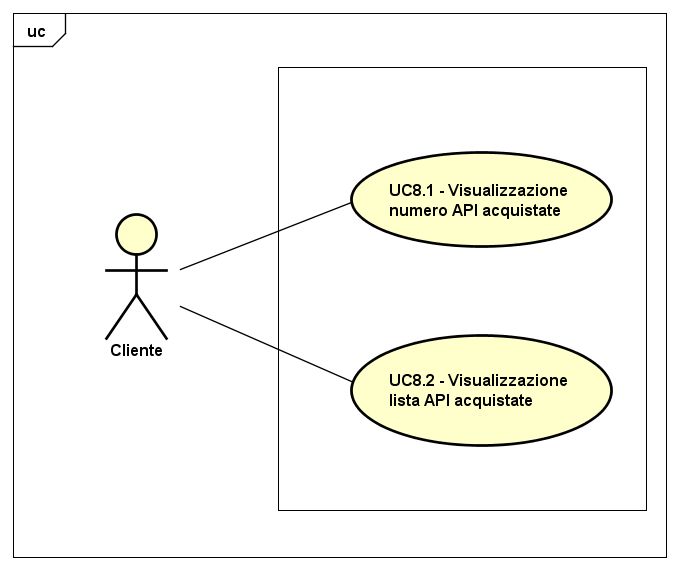
\includegraphics[scale=0.45]{UML/UC8.png}
	\caption{UC8: Visualizzazione API acquistate}
\end{figure}

\begin{longtable}{ l | p{11cm}}
	\hline
	\rowcolor{Gray}
	\multicolumn{2}{c}{UC8 - Visualizzazione API acquistate}\\
	\hline
	 \textbf{Attori} & Cliente \\
	\textbf{Descrizione} & L'attore visualizza le API da lui acquistate \\
	\textbf{Pre-Condizioni} & L'applicazione visualizza la schermata relativa alle API acquistate dal Cliente \\
	\textbf{Post-Condizioni} & L'attore ha visualizzato le API da lui acquistate \\
	\textbf{Scenario Principale} & 
	\begin{enumerate*}[label=(\arabic*.),itemjoin={\newline}]
		\item L'attore può visualizzare il numero delle API acquistate e attive (UC8.1)
		\item L'attore può visualizzare la lista delle API acquistate e attive (UC8.2)
	\end{enumerate*}\\
\end{longtable}

\subsubsection{Caso d'uso UC8.1: Visualizzazione numero API acquistate}
\label{UC8_1}

\begin{minipage}{\linewidth}
	\begin{tabular}{ l | p{11cm}}
		\hline
		\rowcolor{Gray}
		\multicolumn{2}{c}{UC8.1 - Visualizzazione numero API acquistate} \\
		\hline
		\textbf{Attori} & Cliente \\
		\textbf{Descrizione} & L'attore visualizza il numero di API da lui acquistate \\
		\textbf{Pre-Condizioni} & L'attore si trova nella schermata relativa alle API da lui acquistate \\
		\textbf{Post-Condizioni} & L'attore ha visualizzato il numero delle API da lui acquistate \\
		\textbf{Scenario Principale} & 
		\begin{enumerate*}[label=(\arabic*.),itemjoin={\newline}]
			\item L'attore può visualizzare il numero di API acquistate
		\end{enumerate*}\\
	\end{tabular}
\end{minipage}

\newpage
\subsubsection{Caso d'uso UC8.2: Visualizzazione lista API acquistate}
\label{UC8_2}
\begin{figure}[ht]
	\centering
	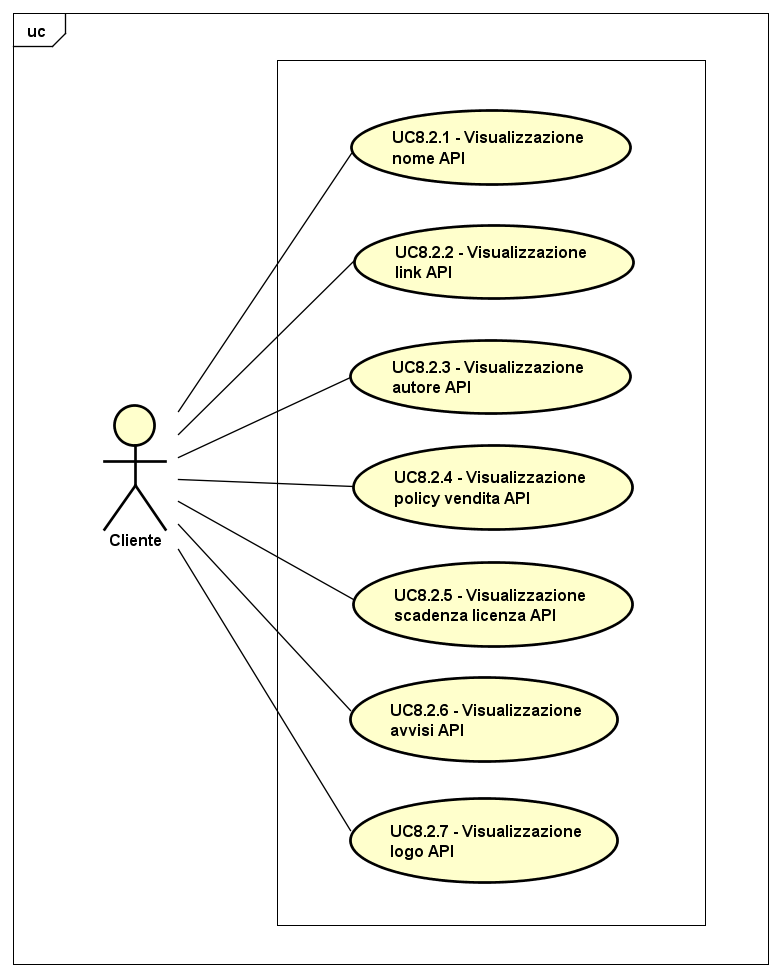
\includegraphics[scale=0.45]{UML/UC8_2.png}
	\caption{UC8.2: Visualizzazione lista API acquistate}
\end{figure}

\begin{minipage}{\linewidth}
	\begin{tabular}{ l | p{11cm}}
		\hline
		\rowcolor{Gray}
		\multicolumn{2}{c}{UC8.2 - Visualizzazione lista API acquistate} \\
		\hline
		\textbf{Attori} & Cliente \\
		\textbf{Descrizione} & L'attore visualizza la lista delle API da lui acquistate \\
		\textbf{Pre-Condizioni} & L'attore si trova nella schermata relativa alle API da lui acquistate \\
		\textbf{Post-Condizioni} & L'attore ha visualizzato la lista delle API da lui acquistate \\
		\textbf{Scenario Principale} & 
		\begin{enumerate*}[label=(\arabic*.),itemjoin={\newline}]
			\item L'attore può visualizzare il nome dell'API (UC8.2.1)
			\item L'attore può visualizzare il link alla pagina di visualizzazione API (UC8.2.2)
			\item L'attore può visualizzare il nome dell'autore dell'API (UC8.2.3)
			\item L'attore può visualizzare la policy di vendita dell'API (UC8.2.4)
			\item L'attore può visualizzare il parametro di scadenza, in base alla policy,  della propria licenza per l'API (UC8.2.5)
			\item L'attore può visualizzare gli avvisi riguardo l'API (UC8.2.6)
			\item L'attore può visualizzare il logo dell'API (UC8.2.7)
		\end{enumerate*}\\
	\end{tabular}
\end{minipage}

\paragraph{Caso d'uso UC8.2.1: Visualizzazione nome API}
\label{UC8_2_1}

\begin{minipage}{\linewidth}
	\begin{tabular}{ l | p{11cm}}
		\hline
		\rowcolor{Gray}
		\multicolumn{2}{c}{UC8.2.1 - Visualizzazione nome API} \\
		\hline
		\textbf{Attori} & Cliente \\
		\textbf{Descrizione} & L'attore visualizza nella lista il nome dell'API \\
		\textbf{Pre-Condizioni} & L'attore si trova nella schermata relativa alle API da lui acquistate \\
		\textbf{Post-Condizioni} & L'attore ha visualizzato nella lista il nome dell'API \\
		\textbf{Scenario Principale} & 
		\begin{enumerate*}[label=(\arabic*.),itemjoin={\newline}]
			\item L'attore può visualizzare nella lista il nome dell'API
		\end{enumerate*}\\
	\end{tabular}
\end{minipage}

\paragraph{Caso d'uso UC8.2.2: Visualizzazione link API}
\label{UC8_2_2}

\begin{minipage}{\linewidth}
	\begin{tabular}{ l | p{11cm}}
		\hline
		\rowcolor{Gray}
		\multicolumn{2}{c}{UC8.2.2 - Visualizzazione link API} \\
		\hline
		\textbf{Attori} & Cliente \\
		\textbf{Descrizione} & L'attore visualizza nella lista il link alla visualizzazione dell'API \\
		\textbf{Pre-Condizioni} & L'attore si trova nella schermata di visualizzazione delle API acquistate \\
		\textbf{Post-Condizioni} & L'attore ha visualizzato nella lista il link alla visualizzazione dell'API \\
		\textbf{Scenario Principale} & 
		\begin{enumerate*}[label=(\arabic*.),itemjoin={\newline}]
			\item L'attore può visualizzare nella lista il link alla visualizzazione dell'API, che lo reindirizzerà ad UC7 per l'API in questione
		\end{enumerate*}\\
	\end{tabular}
\end{minipage}

\paragraph{Caso d'uso UC8.2.3: Visualizzazione nome autore API}
\label{UC8_2_3}

\begin{minipage}{\linewidth}
	\begin{tabular}{ l | p{11cm}}
		\hline
		\rowcolor{Gray}
		\multicolumn{2}{c}{UC8.2.3 - Visualizzazione nome autore API} \\
		\hline
		\textbf{Attori} & Cliente \\
		\textbf{Descrizione} & L'attore visualizza nella lista il nome dell'autore dell'API \\
		\textbf{Pre-Condizioni} & L'attore si trova nella schermata relativa alle API da lui acquistate \\
		\textbf{Post-Condizioni} & L'attore ha visualizzato nella lista il nome dell'autore dell'API \\
		\textbf{Scenario Principale} & 
		\begin{enumerate*}[label=(\arabic*.),itemjoin={\newline}]
			\item L'attore può visualizzare nella lista il nome dell'autore dell'API
		\end{enumerate*}\\
	\end{tabular}
\end{minipage}

\paragraph{Caso d'uso UC8.2.4: Visualizzazione policy vendita API}
\label{UC8_2_4}

\begin{minipage}{\linewidth}
	\begin{tabular}{ l | p{11cm}}
		\hline
		\rowcolor{Gray}
		\multicolumn{2}{c}{UC8.2.4 - Visualizzazione policy vendita API} \\
		\hline
		\textbf{Attori} & Cliente \\
		\textbf{Descrizione} & L'attore visualizza nella lista la policy di vendita dell'API \\
		\textbf{Pre-Condizioni} & L'attore si trova nella schermata relativa alle API da lui acquistate \\
		\textbf{Post-Condizioni} & L'attore ha visualizzato nella lista la policy di vendita dell'API \\
		\textbf{Scenario Principale} & 
		\begin{enumerate*}[label=(\arabic*.),itemjoin={\newline}]
			\item L'attore può visualizzare nella lista la policy di vendita dell'API
		\end{enumerate*}\\
	\end{tabular}
\end{minipage}

\paragraph{Caso d'uso UC8.2.5: Visualizzazione scadenza licenza}
\label{UC8_2_5}

\begin{minipage}{\linewidth}
	\begin{tabular}{ l | p{11cm}}
		\hline
		\rowcolor{Gray}
		\multicolumn{2}{c}{UC8.2.3 - Visualizzazione scadenza licenza} \\
		\hline
		\textbf{Attori} & Cliente \\
		\textbf{Descrizione} & L'attore visualizza nella lista la data di scadenza della propria licenza per l'API \\
		\textbf{Pre-Condizioni} & L'attore si trova nella schermata relativa alle API da lui acquistate \\
		\textbf{Post-Condizioni} & L'attore ha visualizzato nella lista il parametro di scadenza dell'API \\
		\textbf{Scenario Principale} & 
		\begin{enumerate*}[label=(\arabic*.),itemjoin={\newline}]
			\item L'attore può visualizzare nella lista il parametro di scadenza della propria licenza per l'API
		\end{enumerate*}\\
	\end{tabular}
\end{minipage}

\paragraph{Caso d'uso UC8.2.6: Visualizzazione avvisi API}
\label{UC8_2_6}

\begin{minipage}{\linewidth}
	\begin{tabular}{ l | p{11cm}}
		\hline
		\rowcolor{Gray}
		\multicolumn{2}{c}{UC8.2.6 - Visualizzazione avvisi API} \\
		\hline
		\textbf{Attori} & Cliente \\
		\textbf{Descrizione} & L'attore visualizza nella lista gli avvisi riguardanti l'API \\
		\textbf{Pre-Condizioni} & L'attore si trova nella schermata relativa alle API da lui acquistate \\
		\textbf{Post-Condizioni} & L'attore ha visualizzato nella lista gli avvisi riguardanti l'API \\
		\textbf{Scenario Principale} & 
		\begin{enumerate*}[label=(\arabic*.),itemjoin={\newline}]
			\item L'attore può visualizzare nella lista gli avvisi riguardanti l'API (E.g: cancellazione, manutenzione)
		\end{enumerate*}\\
	\end{tabular}
\end{minipage}

\paragraph{Caso d'uso UC8.2.7: Visualizzazione logo API}
\label{UC8_2_7}

\begin{minipage}{\linewidth}
	\begin{tabular}{ l | p{11cm}}
		\hline
		\rowcolor{Gray}
		\multicolumn{2}{c}{UC8.2.7 - Visualizzazione logo API} \\
		\hline
		\textbf{Attori} & Cliente \\
		\textbf{Descrizione} & L'attore visualizza nella lista il logo dell'API \\
		\textbf{Pre-Condizioni} & L'attore si trova nella schermata relativa alle API da lui acquistate \\
		\textbf{Post-Condizioni} & L'attore ha visualizzato nella lista il logo dell'API \\
		\textbf{Scenario Principale} & 
		\begin{enumerate*}[label=(\arabic*.),itemjoin={\newline}]
			\item L'attore può visualizzare nella lista il logo dell'API
		\end{enumerate*}\\
	\end{tabular}
\end{minipage}